\documentclass[a4paper,10pt]{book}
\usepackage[utf8]{inputenc}
\usepackage{tikz}
\usepackage{hyperref}

\newcommand{\icon}[1]{\tikz[baseline=-3pt] \node[inner sep=0pt,outer sep=0pt]{\includegraphics[height=1.1em]{images/#1}};}

%opening
\title{ADAMS - Scientific Workflow Management}
\author{Peter Reutemann}

\begin{document}

\chapter{Twitter Research}
ADAMS offers a large amount of actors for a wide range of data processing and mining tasks. However, we limit ourselves here to the analysis of data obtained from Twitter. The following sections cover how to set up ADAMS in order to access Twitter, how to collect tweets for further (and repeated) analysis, replay previously collected tweets, visualize tweets and how to perform various analyses.

\section{Twitter setup}
ADAMS uses the twitter4j\footnote{\url{http://twitter4j.org/}{}} library for accessing twitter. In order to access some of the functionality of the Twitter API, you need to have a developer account and register an application with API key/secret and Access token/secret. You can register an application on the Twitter Developer website\footnote{\url{https://dev.twitter.com/}{}}. Figure \ref{twitter_dev} shows an example website for an ADAMS application, complete with generated API key/secret and Access token/secret. Once you have obtained these keys/tokens/secrets you can enter these in the ADAMS preferences for Twitter, as shown in Figure \ref{twitter_preferences}. These preferences are global and get picked up by the \icon{TwitterConnection}~TwitterConnection actor as default values, which you can always override, in case you need different credentials.

\begin{figure}[htb]
  \centering
  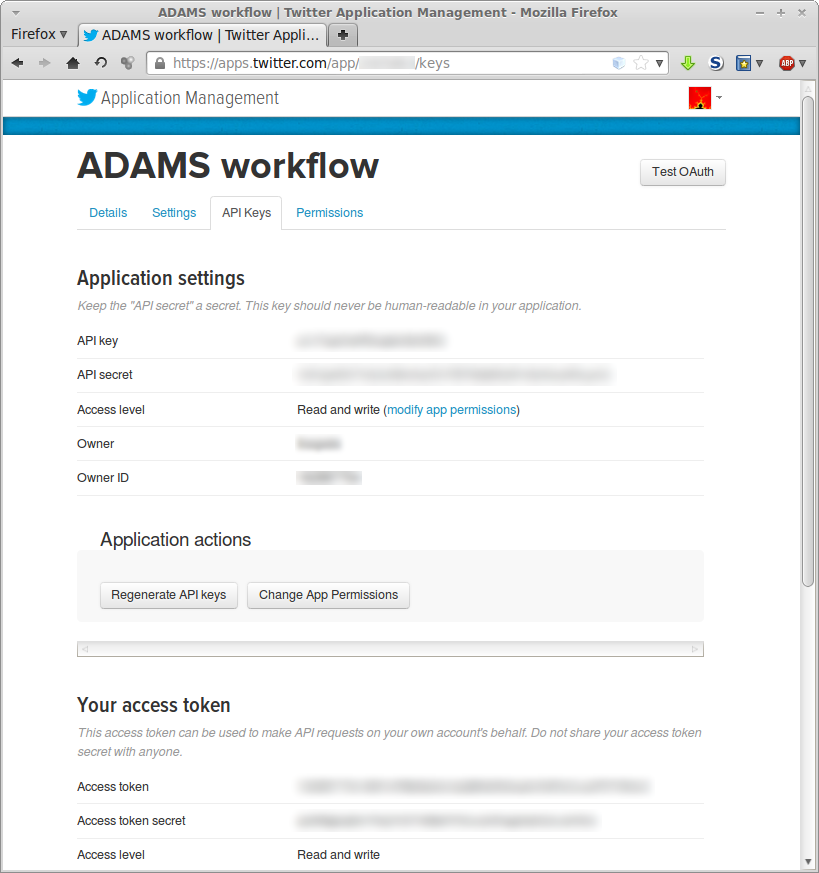
\includegraphics[width=10.0cm]{images/twitter_dev.png}
  \caption{Application management through the ``Twitter Developers'' website, displaying keys, tokens and secrets for an application.}
  \label{twitter_dev}
\end{figure}

\begin{figure}[htb]
  \centering
  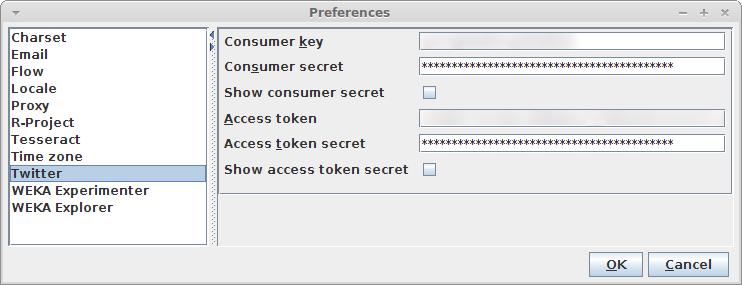
\includegraphics[width=10.0cm]{images/twitter_preferences.png}
  \caption{Preferences page for Twitter in ADAMS.}
  \label{twitter_preferences}
\end{figure}

\clearpage
\newpage
\section{Collecting tweets}
Rather than just obtaining the tweets of a single user, Twitter allows you to tap into the stream of tweets as they are posted in real-time using their streaming API\footnote{\url{https://dev.twitter.com/docs/streaming-apis}{}}. However, Twitter distinguishes between the ``fire hose'' and the ``garden hose''. The former being the complete stream of tweets, which is only accessible to paying customers that have sufficient bandwidth and hardware to cope with the flood of information. The latter is a 1\% sample of the complete stream, which available to the public. The ``garden hose'' is what can be accessed using ADAMS.

According to Twitter's API Rules, you can collect tweets, but you are not allowed to redistribute them.\footnote{See \url{https://twitter.com/apirules}{} for more details.} ADAMS therefore fills the void of publicly available tweet archives, by allowing you to collect a large corpus of tweets yourself. You simply set up a flow for collecting tweets and let it run for a number of days, weeks or even months.

In order to collect tweets, you basically only need the following three actors:
\begin{itemize}
  \item \icon{TwitterConnection}~\textbf{TwitterConnection} -- for connecting to Twitter.
  \item \icon{TwitterListener}~\textbf{TwitterListener} -- for accessing the ``garden hose'' stream of tweets.
  \item \icon{TwitterConverter}~\textbf{TwitterConverter} -- for turning the tweets into a data format suitable for future analysis, e.g., spreadsheet format.
\end{itemize}
Unless you are storing the data in a database, the generated tweet archive file will get rather large, since there are several million tweets coming through the ``garden hose'' every single day. The flow depicted in Figure \ref{collect_tweets-flow} saves the tweets in a special ADAMS CSV (comma-separated values) file format, which can be used for replaying the tweets again. In order to avoid too large an output file, the tweets get grouped by day. 

The flow works as follows:
\begin{itemize}
  \item Since we need the file name generation more than once in the flow and we do not want to duplicate the functionality, we push the generation into \icon{CallableActors}~CallableActors, which basically acts as a function call. The file name generation consists of several steps, i.e., we need to encapsulate them in a \icon{SequenceSource}~SequenceSource called ``filename''.
  
  \item The \icon{TwitterListener}~TwitterListener source is configured to output an unlimited number of tweets, i.e., the user needs to explicitly stop the flow before the collection of tweets finishes.
  
  \item To begin with, the \icon{Once}~Once control actor\footnote{As the name suggests, the \textit{Once} actor triggers its nested actors only with the first token passing through, as opposed to the default \textit{Trigger} actor which executes its nested actors each time a token passes through.} initializes the variable obtaining the current file name by executing the callable actor ``filename'' through the \icon{CallableSource}~CallableSource source actor and setting the variable with the \icon{SetVariable}~SetVariable actor.

  \item Every 1000 tweets, the \icon{ConditionalTrigger}~ConditionalTrigger control actor executes its nested actors, checking whether a newly generate CSV file name differs from the one currently stored in the variable \texttt{@\{filename\}}.
    \begin{itemize}
      \item Should that be the case, i.e., the \icon{ConditionalTee}~ConditionalTee actor evaluates to true, the variable \texttt{@\{filename\}} gets updated using the \icon{SetVariable}~SetVariable transformer.
    \end{itemize}
  
  \item Each tweet gets converted into a spreadsheet object using the \icon{TwitterConverter}~TwitterConverter transformer, selecting all data fields deemed important.
  
  \item The generated spreadsheet object then gets stored in the CSV file with the \icon{SpreadSheetFileWriter}~SpreadSheetFileWriter sink, using the current file name stored in the variable \texttt{@\{filename\}}.
\end{itemize}


\begin{figure}[htb]
  \centering
  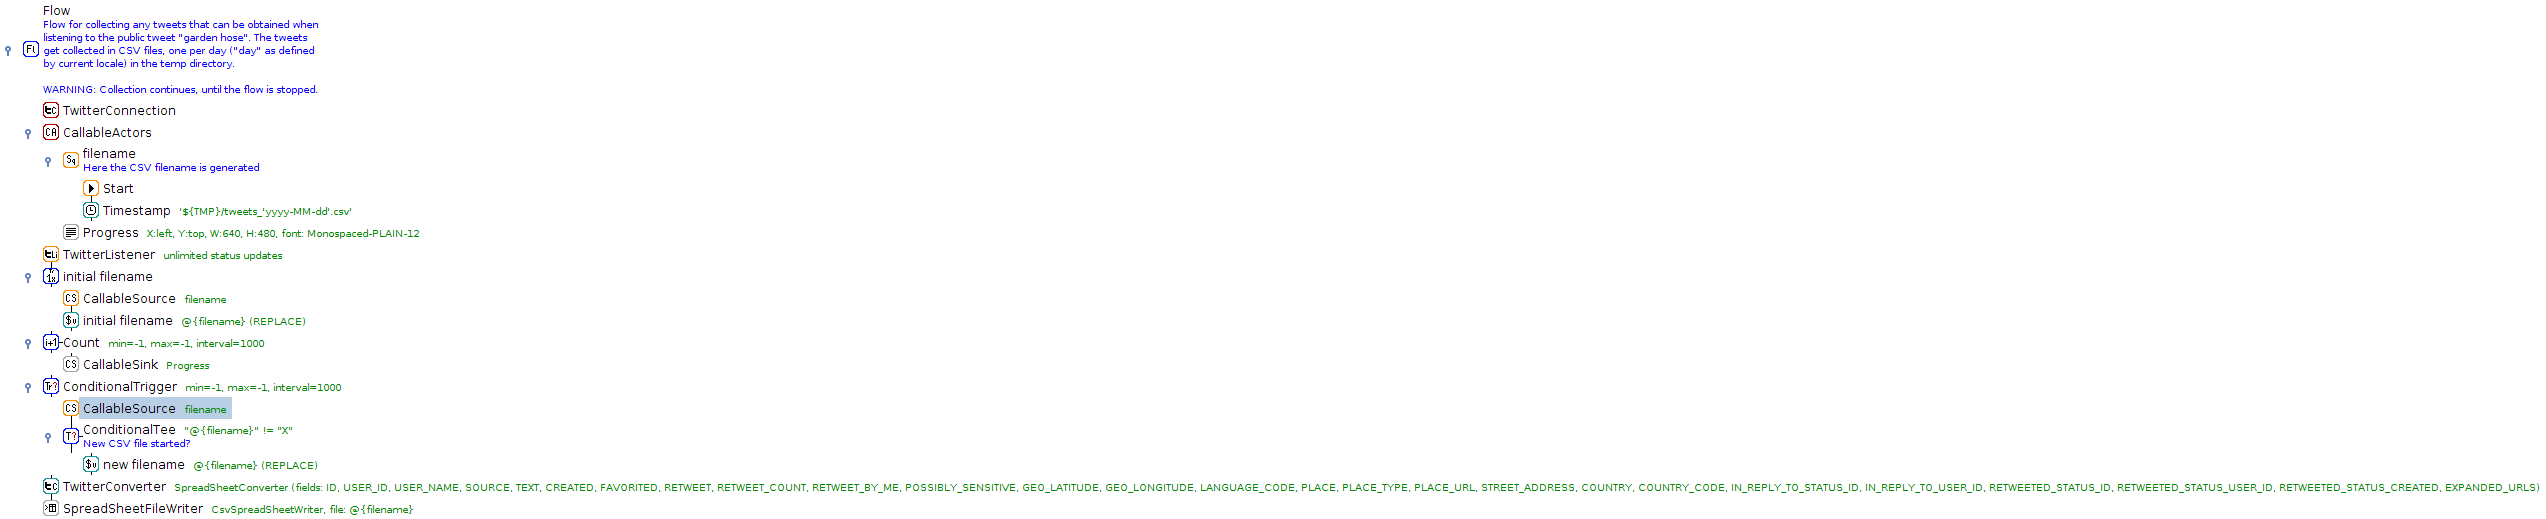
\includegraphics[width=8.0cm]{images/collect_tweets-flow.png}
  \caption{Flow for collecting tweets in CSV archive files.}
  \label{collect_tweets-flow}
\end{figure}

\clearpage
\newpage
\section{Replaying and filtering tweets}
TODO

\begin{figure}[htb]
  \centering
  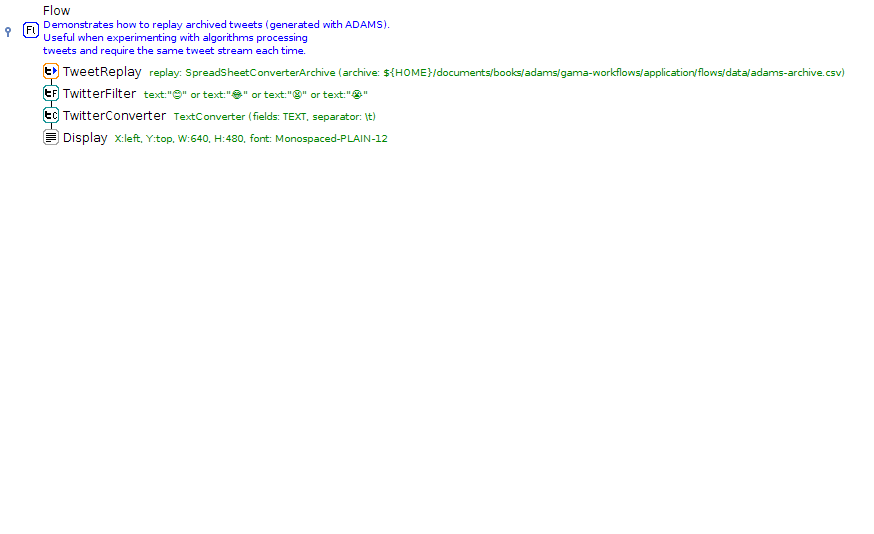
\includegraphics[width=10.0cm]{images/replay_and_filter_tweets-flow.png}
  \caption{Flow for replaying and filtering tweets from a CSV archive, using simple textual output.}
  \label{replay_and_filter_tweets-flow}
\end{figure}

\begin{figure}[htb]
  \centering
  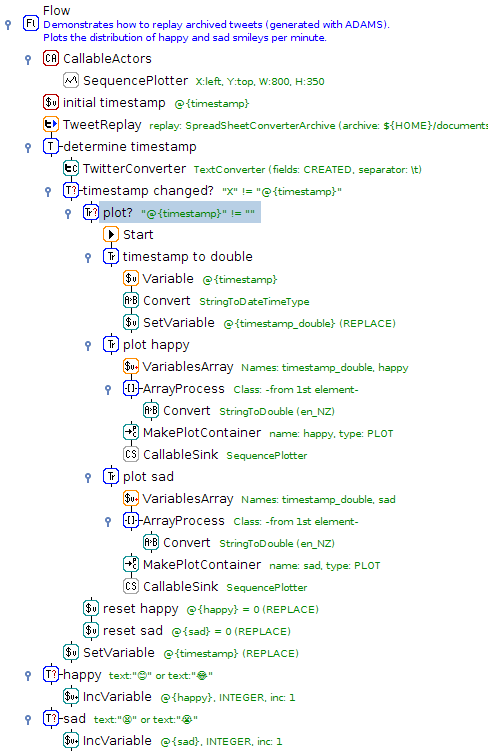
\includegraphics[width=8.0cm]{images/replay_and_filter_tweets2-flow.png}
  \caption{Flow for replaying and filtering tweets from a CSV archive, displaying mood distribution per minute.}
  \label{replay_and_filter_tweets2-flow}
\end{figure}

\begin{figure}[htb]
  \centering
  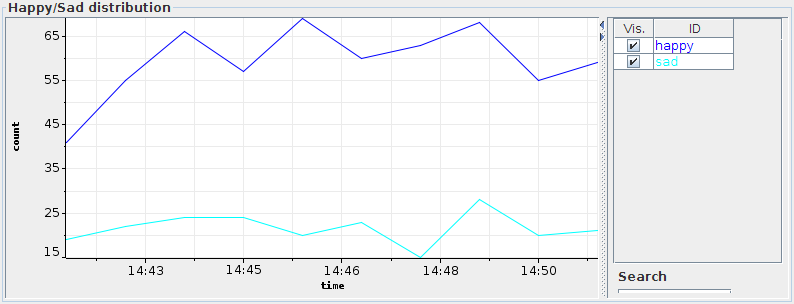
\includegraphics[width=10.0cm]{images/replay_and_filter_tweets2-output.png}
  \caption{Visualization of mood distribution per minute (``happy'' and ``sad'' smiley counts).}
  \label{replay_and_filter_tweets2-output}
\end{figure}

\begin{figure}[htb]
  \centering
  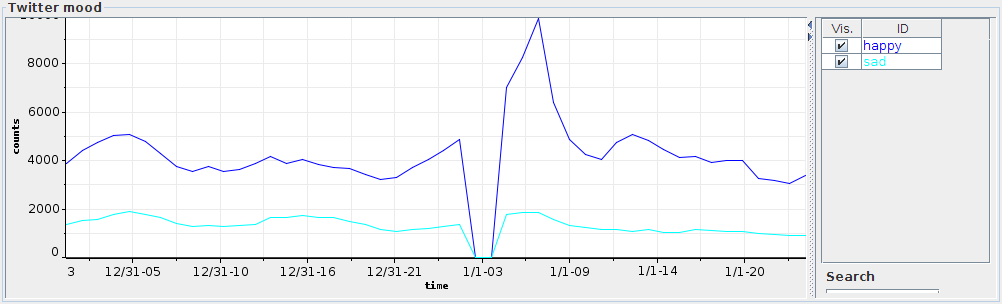
\includegraphics[width=10.0cm]{images/twitter_mood.png}
  \caption{Visualization of mood distribution per hour over New Years 2013/2014 (``happy'' and ``sad'' smiley counts).}
  \label{twitter_mood}
\end{figure}

\clearpage
\newpage
\section{Visualizing tweets}
TODO

\subsection{Analysis}
TODO

\begin{figure}[htb]
  \centering
  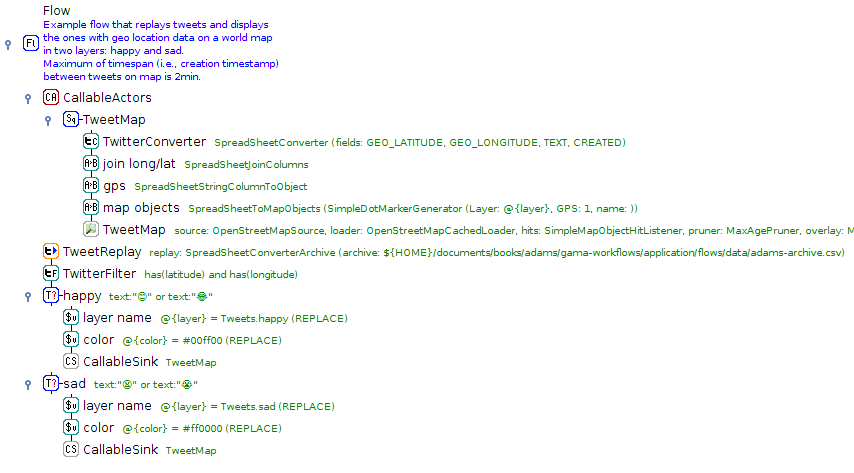
\includegraphics[width=12.0cm]{images/visualize_tweets-archive-flow.png}
  \caption{Flow for visualizing tweets archive.}
  \label{visualize_tweets-archive-flow}
\end{figure}

\begin{figure}[htb]
  \centering
  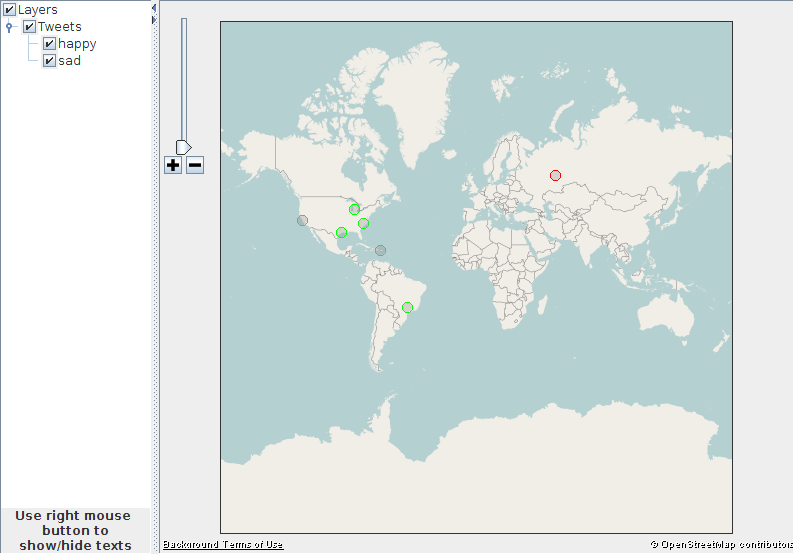
\includegraphics[width=10.0cm]{images/visualize_tweets-archive-output.png}
  \caption{Flow for visualizing tweets archive.}
  \label{visualize_tweets-archive-output}
\end{figure}

\subsection{Real-time visualization}
TODO

\begin{figure}[htb]
  \centering
  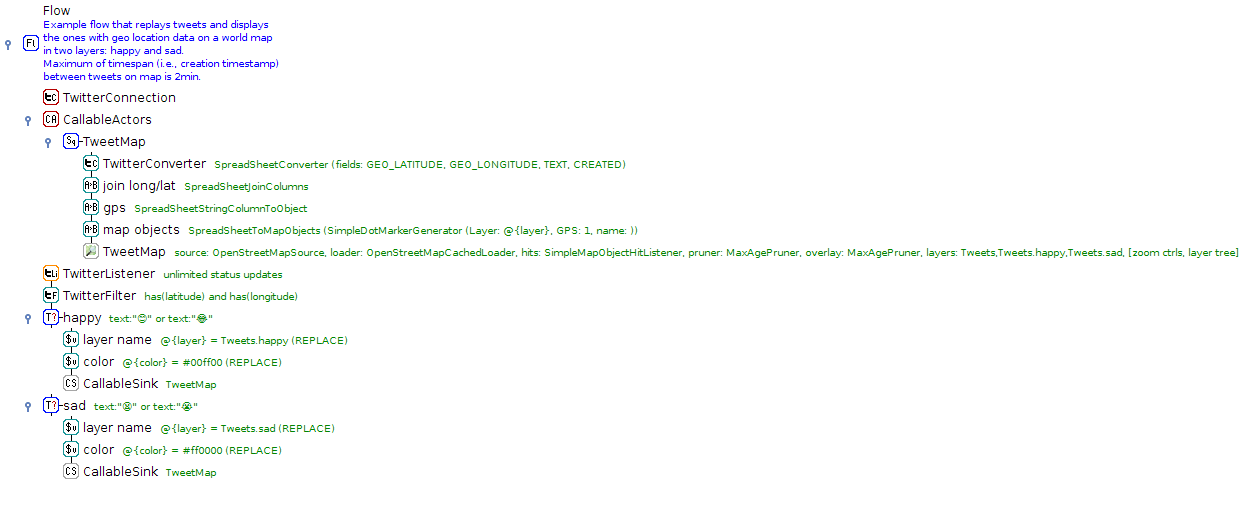
\includegraphics[width=12.0cm]{images/visualize_tweets-realtime-flow.png}
  \caption{Flow for visualizing tweets in real-time.}
  \label{visualize_tweets-realtime-flow}
\end{figure}

\end{document}
